\chapter{Metric Spaces}

\section{Distance}

\begin{definition}[Metric]
A \emph{metric} on a set $X$ is a function $d : X \times X \to \R$ such that for all $x, y, z \in X$:
\begin{enumerate}
  \item $\dist{x}{y} \ge 0$, with equality exactly when $x = y$;
  \item $\dist{x}{y} = \dist{y}{x}$;
  \item $\dist{x}{z} \le \dist{x}{y} + \dist{y}{z}$.
\end{enumerate}
\end{definition}

\begin{example}
On $\R$, $\dist{x}{y} = \abs{x - y}$ is a metric.
\end{example}

\begin{center}
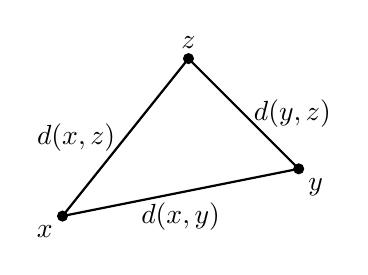
\begin{tikzpicture}
  \coordinate (x) at (0,0); \coordinate (y) at (3,0.6); \coordinate (z) at (1.6,2);
  \draw[thick] (x) -- node[below] {$d(x,y)$} (y) -- node[right] {$d(y,z)$} (z) -- node[left] {$d(x,z)$} (x);
  \foreach \p in {x,y,z} \fill (\p) circle (2pt);
  \node[below left] at (x) {$x$}; \node[below right] at (y) {$y$}; \node[above] at (z) {$z$};
\end{tikzpicture}
\end{center}

\begin{important}[Triangle inequality]
Going through a third point is never shorter: $\dist{x}{z} \le \dist{x}{y} + \dist{y}{z}$.
\end{important}
